\chapter{Exercise 2}

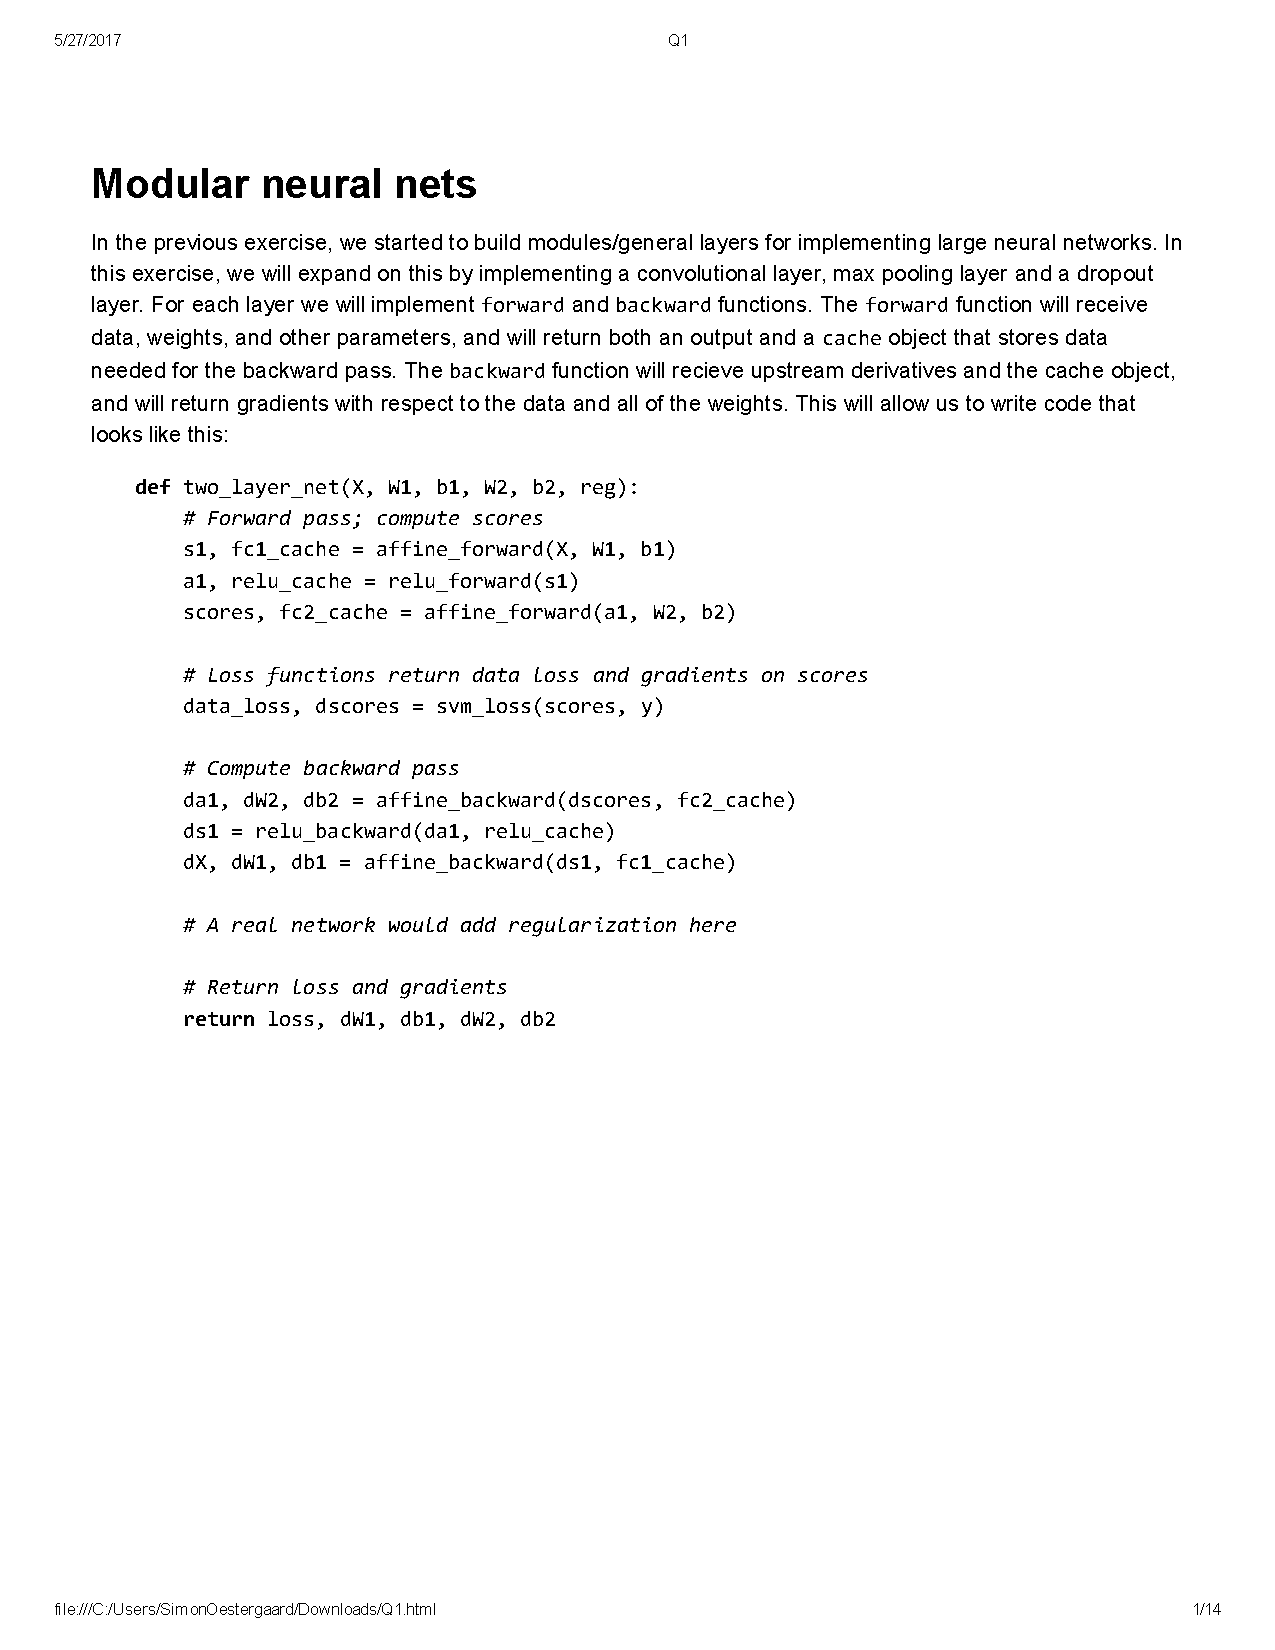
\includepdf[pages={-}]{chapter/2_Q1.pdf}


\begin{lstlisting}[language=Python, label=lst:layers.py, caption={layers.py}, basicstyle=\tiny]
import numpy as np

def affine_forward(x, w, b):
"""
Computes the forward pass for an affine (fully-connected) layer.

The input x has shape (N, d_1, ..., d_k) where x[i] is the ith input.
We multiply this against a weight matrix of shape (D, M) where
D = \prod_i d_i

Inputs:
x - Input data, of shape (N, d_1, ..., d_k)
w - Weights, of shape (D, M)
b - Biases, of shape (M,)

Returns a tuple of:
- out: output, of shape (N, M)
- cache: (x, w, b)
"""
out = None
#############################################################################
# TODO: Implement the affine forward pass. Store the result in out. You     #
# will need to reshape the input into rows.                                 #
#############################################################################
# First we reshape X to mulitply it with the incoming weights
# We get column and row size and then reshape
row_size = x.shape[0]
col_size = np.prod(x.shape[1:])
x_reshape = x.reshape(row_size, col_size)
# Then to execute the forward pass we simply need to multiply the
# inputs with the weights
out = np.dot(x_reshape, w) + b
#############################################################################
#                             END OF YOUR CODE                              #
#############################################################################
cache = (x, w, b)
return out, cache


def affine_backward(dout, cache):
"""
Computes the backward pass for an affine layer.

Inputs:
- dout: Upstream derivative, of shape (N, M)
- cache: Tuple of:
- x: Input data, of shape (N, d_1, ... d_k)
- w: Weights, of shape (D, M)

Returns a tuple of:
- dx: Gradient with respect to x, of shape (N, d1, ..., d_k)
- dw: Gradient with respect to w, of shape (D, M)
- db: Gradient with respect to b, of shape (M,)
"""
x, w, b = cache
dx, dw, db = None, None, None
#############################################################################
# TODO: Implement the affine backward pass.                                 #
#############################################################################
# First we reshape X to mulitply it with the incoming weights
# We get column and row size and then reshape
row_size = x.shape[0]
col_size = np.prod(x.shape[1:])
x_reshape = x.reshape(row_size, col_size)

# After reshaping we calculate the backward pass

# Gradient with respect to x
# Gradient of x*w with respect to x is simply w, so we multiply that 
# with the upstream gradient
dx2 = np.dot(dout, w.T) 
dx = np.reshape(dx2, x.shape)

# Gradient with respect to weights
# # Gradient of x*w with respect to w is simply x, 
# so we multiply that with the upstream gradient
dw = np.dot(x_reshape.T, dout)

# Gradient with respect to bias
# Biases are added so the gradient is simply 1, 
# so we multiply that with the upstream gradient.
db = np.dot(dout.T, np.ones(row_size))

#############################################################################
#                             END OF YOUR CODE                              #
#############################################################################
return dx, dw, db


def relu_forward(x):
"""
Computes the forward pass for a layer of rectified linear units (ReLUs).

Input:
- x: Inputs, of any shape

Returns a tuple of:
- out: Output, of the same shape as x
- cache: x
"""
out = None
#############################################################################
# TODO: Implement the ReLU forward pass.                                    #
#############################################################################
reluF = lambda x: np.maximum(0, x)
out = reluF(x)
#############################################################################
#                             END OF YOUR CODE                              #
#############################################################################
cache = x
return out, cache


def relu_backward(dout, cache):
"""
Computes the backward pass for a layer of rectified linear units (ReLUs).

Input:
- dout: Upstream derivatives, of any shape
- cache: Input x, of same shape as dout

Returns:
- dx: Gradient with respect to x
"""
dx, x = None, cache
#############################################################################
# TODO: Implement the ReLU backward pass.                                   #
#############################################################################
#reluf function
reluF = lambda x: np.maximum(0, x)

out = reluF(x)
# Reluf is a max gate and so we can think of it as a router of gradients
# the max value is the one that the gradient is routated to
# we simpy set the out value to 1 if the out value is bigger than 0
out[out > 0] = 1

# Multiply out  with upstream gradient, to "route" the gradient
dx = out * dout
#############################################################################
#                             END OF YOUR CODE                              #
#############################################################################
return dx

def dropout_forward(x, dropout_param):
"""
Performs the forward pass for (inverted) dropout.

Inputs:
- x: Input data, of any shape
- dropout_param: A dictionary with the following keys:
- p: Dropout parameter. We keep each neuron output with probability p.
- mode: 'test' or 'train'. If the mode is train, then perform dropout;
if the mode is test, then just return the input.
- seed: Seed for the random number generator. Passing seed makes this
function deterministic, which is needed for gradient checking but not in
real networks.

Outputs:
- out: Array of the same shape as x.
- cache: A tuple (dropout_param, mask). In training mode, mask is the dropout
mask that was used to multiply the input; in test mode, mask is None.
"""
p, mode = dropout_param['p'], dropout_param['mode']
if 'seed' in dropout_param:
np.random.seed(dropout_param['seed'])

mask = None
out = None

if mode == 'train':
###########################################################################
# TODO: Implement the training phase forward pass for inverted dropout.   #
# Store the dropout mask in the mask variable.                            #
###########################################################################
# mask is equal to random 
# random creates uniform distribution between 0 and 1.
# If the value is less than p then we set it equals 0 and if not we set it equals 1
# We divide to get inverted, so the ones wich evaluates to 1 gets a higher value
mask = (np.random.rand(*x.shape) < p) / p
# by multiplying the input with the mask we deactive some neurons
out = x * mask
###########################################################################
#                            END OF YOUR CODE                             #
###########################################################################
elif mode == 'test':
###########################################################################
# TODO: Implement the test phase forward pass for inverted dropout.       #
###########################################################################
out = x
###########################################################################
#                            END OF YOUR CODE                             #
###########################################################################

cache = (dropout_param, mask)
out = out.astype(x.dtype, copy=False)

return out, cache


def dropout_backward(dout, cache):
"""
Perform the backward pass for (inverted) dropout.

Inputs:
- dout: Upstream derivatives, of any shape
- cache: (dropout_param, mask) from dropout_forward.
"""
dropout_param, mask = cache
mode = dropout_param['mode']
if mode == 'train':
###########################################################################
# TODO: Implement the training phase backward pass for inverted dropout.   #
# Store the dropout mask in the mask variable.                            #
###########################################################################
# we only backpropagate the acitivated neurons
dx = dout*mask
###########################################################################
#                            END OF YOUR CODE                             #
###########################################################################
elif mode == 'test':
dx = dout
return dx


def conv_forward_naive(x, w, b, conv_param):
"""
A naive implementation of the forward pass for a convolutional layer.

The input consists of N data points, each with C channels, height H and width
W. We convolve each input with F different filters, where each filter spans
all C channels and has height HH and width HH.

Input:
- x: Input data of shape (N, C, H, W)
- w: Filter weights of shape (F, C, HH, WW)
- b: Biases, of shape (F,)
- conv_param: A dictionary with the following keys:
- 'stride': The number of pixels between adjacent receptive fields in the
horizontal and vertical directions.
- 'pad': The number of pixels that will be used to zero-pad the input.

Returns a tuple of:
- out: Output data, of shape (N, F, H', W') where H' and W' are given by
H' = 1 + (H + 2 * pad - HH) / stride
W' = 1 + (W + 2 * pad - WW) / stride
- cache: (x, w, b, conv_param)
"""
out = None
#############################################################################
# TODO: Implement the convolutional forward pass.                           #
# Hint: you can use the function np.pad for padding.                        #
#############################################################################
#  N(data points), C(channels), H(height), W(Width)
N, C, H, W = x.shape
# F (diffferent filters), C(channels), HH ( channel height), WW(channel width)
F, C, HH, WW = w.shape
# number of pixels that will be used to zero-pad inud
pad = conv_param['pad']
#Stride
stride = conv_param['stride']
# Formula for h prime and w prime are given above
H_prime = 1 + (H + 2 * pad - HH) / stride
W_prime = 1 + (W + 2 * pad - WW) / stride
# This is the shape of out, we initialize to all zeroes
out = np.zeros((N, F, H_prime, W_prime))

# padding
#numpy.pad(array, pad_width, mode, **kwargs)
x_with_pad = np.pad(x, ((0,0),(0,0),(pad,pad),(pad,pad)), 'constant', constant_values=0)
#Width an height of input including zero padding
_, _, H, W = x_with_pad.shape

# convolution
# running N iterations, one iteration for each data point
for n in range(N):
#Extract the ith row of x_with_bad
x_pad = x_with_pad[n]
# run iteration for each filter
for f in range(F):
#run iteration corresponding to the height of the output
for h_prime in range(H_prime):
#run iteration corresponding to the width of the output
for w_prime in range(W_prime):
# bottom height
h1 = h_prime * stride
# top height (by adding channel height)
h2 = h_prime * stride + HH
# start width
w1 = w_prime * stride
# end width ( by adding channel width)
w2 = w_prime * stride + WW
# the window is the x_padded from h1 to h2 and w1-w2 to get the window
window = x_pad[:, h1:h2, w1:w2]
# Output data has shape (N, F, H', W') 
# we insert on n (datapoint) f(filter), h_prime and w_prime, 
# The output is sum of the window times the filter weight for f + the bias for f
out[n, f, h_prime, w_prime] = np.sum(window * w[f,:,:,:]) + b[f]
#############################################################################
#                             END OF YOUR CODE                              #
#############################################################################
cache = (x, w, b, conv_param)
return out, cache


def conv_backward_naive(dout, cache):
"""
A naive implementation of the backward pass for a convolutional layer.

Inputs:
- dout: Upstream derivatives.
- cache: A tuple of (x, w, b, conv_param) as in conv_forward_naive

Returns a tuple of:
- dx: Gradient with respect to x
- dw: Gradient with respect to w
- db: Gradient with respect to b
"""
dx, dw, db = None, None, None
#############################################################################
# TODO: Implement the convolutional backward pass.                          #
#############################################################################
x, w, b, conv_param = cache
#  N(data points), C(channels), H(height), W(Width)
N, C, H, W = x.shape
# F (diffferent filters), C(channels), HH ( channel height), WW(channel width)
F, C, HH, WW = w.shape
# shape of upstream derivatives
_, _, H_prime, W_prime = dout.shape
# number of pixels that will be used to zero-pad inud
pad = conv_param['pad']
#Stride
stride = conv_param['stride']

# array of shame shape and type
dx = np.zeros_like(x)
dw = np.zeros_like(w)
db = np.zeros_like(b)

# iterate for each datapoints
for n in xrange(N):   
#Zero padding for dx and x
dx_pad = np.pad(dx[n,:,:,:], ((0,0),(pad,pad),(pad,pad)), 'constant')
x_pad = np.pad(x[n,:,:,:], ((0,0),(pad,pad),(pad,pad)), 'constant')
#Backpropagate for each filter
for f in xrange(F):
#for height and width of output data of forward pass
for h_prime in xrange(H_prime):
for w_prime in xrange(W_prime):
#Get window size
# start height
h1 = h_prime * stride
# end height ( plus channel height)
h2 = h_prime * stride + HH
# start width
w1 = w_prime * stride
# end width (plus channel width)
w2 = w_prime * stride + WW
# gradient for x padded and multiply with upstream
dx_pad[:, h1:h2, w1:w2] += w[f,:,:,:] * dout[n,f,h_prime,w_prime]
# Calculate gradient for weights and multiply withn upstream
dw[f,:,:,:] += x_pad[:, h1:h2, w1:w2] * dout[n,f,h_prime,w_prime]
#Calculate gradients for bias and multiply with upstream
db[f] += dout[n,f,h_prime,w_prime]
#Set gradient of x based on gradient on x with padding.
dx[n,:,:,:] = dx_pad[:,1:-1,1:-1]

#############################################################################
#                             END OF YOUR CODE                              #
#############################################################################
return dx, dw, db


def max_pool_forward_naive(x, pool_param):
"""
A naive implementation of the forward pass for a max pooling layer.

Inputs:
- x: Input data, of shape (N, C, H, W)
- pool_param: dictionary with the following keys:
- 'pool_height': The height of each pooling region
- 'pool_width': The width of each pooling region
- 'stride': The distance between adjacent pooling regions

Returns a tuple of:
- out: Output data
- cache: (x, pool_param)
"""
out = None
#############################################################################
# TODO: Implement the max pooling forward pass                              #
#############################################################################
#  N(data points), C(channels), H(height), W(Width)
N, C, H, W = x.shape
# Extract pool height, pool width and stride
pool_height = pool_param['pool_height']
pool_width = pool_param['pool_width']
stride = pool_param['stride']
# New height width can be calculated after pooling
# as the formula below for height 32 and 2x2 pooling and stride of 2 
# this would for example equal 16
H_prime = 1 + (H - pool_height) / stride
W_prime = 1 + (W - pool_width) / stride

# The size of the output. Datapoints with C channels of the new height and width
out = np.zeros((N, C, H_prime, W_prime))

# for all datapoints
for n in xrange(N):
# For the range of the height and width
for h in xrange(H_prime):
for w in xrange(W_prime):
# define pooling window
h1 = h * stride
h2 = h * stride + pool_height
w1 = w * stride
w2 = w * stride + pool_width
#Extract window from data input x for data point n
window = x[n, :, h1:h2, w1:w2]
# Take max and insert it out
out[n,:,h,w] = np.max(window.reshape((C, pool_height*pool_width)), axis=1)
#############################################################################
#                             END OF YOUR CODE                              #
#############################################################################
cache = (x, pool_param)
return out, cache


def max_pool_backward_naive(dout, cache):
"""
A naive implementation of the backward pass for a max pooling layer.

Inputs:
- dout: Upstream derivatives
- cache: A tuple of (x, pool_param) as in the forward pass.

Returns:
- dx: Gradient with respect to x
"""
dx = None
#############################################################################
# TODO: Implement the max pooling backward pass                             #
#############################################################################
x, pool_param = cache
# N(data points), C(channels), H(height), W(Width)
N, C, H, W = x.shape
# Extract pool height, pool width and stride
pool_height = pool_param['pool_height']
pool_width = pool_param['pool_width']
stride = pool_param['stride']
# New height width can be calculated after pooling
# as the formula below for height 32 and 2x2 pooling and stride of 2 
# this would for example equal 16
H_prime = 1 + (H - pool_height) / stride
W_prime = 1 + (W - pool_width) / stride

# Create output gradient of same size as x
dx = np.zeros_like(x)

# iterate through all data points
for n in xrange(N):
#Al channesl
for c in xrange(C):
#And for every height and width pixel
for h in xrange(H_prime):
for w in xrange(W_prime):
#Calculate pooling window
h1 = h * stride
h2 = h * stride + pool_height
w1 = w * stride
w2 = w * stride + pool_width
#extract window
window = x[n, c, h1:h2, w1:w2]
# Find max in window and set to one and rest to zeroes
# Remember that max distributes gradient, so only the max "gets" the gradient
window2 = np.reshape(window, (pool_height*pool_width))
window3 = np.zeros_like(window2)
window3[np.argmax(window2)] = 1
# reshape window 3 with pool window size and  multiply with upstream gradient
dx[n,c,h1:h2,w1:w2] = np.reshape(window3,(pool_height,pool_width)) * dout[n,c,h,w]
#############################################################################
#                             END OF YOUR CODE                              #
#############################################################################
return dx


def svm_loss(x, y):
"""
Computes the loss and gradient using for multiclass SVM classification.

Inputs:
- x: Input data, of shape (N, C) where x[i, j] is the score for the jth class
for the ith input.
- y: Vector of labels, of shape (N,) where y[i] is the label for x[i] and
0 <= y[i] < C

Returns a tuple of:
- loss: Scalar giving the loss
- dx: Gradient of the loss with respect to x
"""
N = x.shape[0]
correct_class_scores = x[np.arange(N), y]
margins = np.maximum(0, x - correct_class_scores[:, np.newaxis] + 1.0)
margins[np.arange(N), y] = 0
loss = np.sum(margins) / N
num_pos = np.sum(margins > 0, axis=1)
dx = np.zeros_like(x)
dx[margins > 0] = 1
dx[np.arange(N), y] -= num_pos
dx /= N
return loss, dx


def softmax_loss(x, y):
"""
Computes the loss and gradient for softmax classification.

Inputs:
- x: Input data, of shape (N, C) where x[i, j] is the score for the jth class
for the ith input.
- y: Vector of labels, of shape (N,) where y[i] is the label for x[i] and
0 <= y[i] < C

Returns a tuple of:
- loss: Scalar giving the loss
- dx: Gradient of the loss with respect to x
"""
probs = np.exp(x - np.max(x, axis=1, keepdims=True))
probs /= np.sum(probs, axis=1, keepdims=True)
N = x.shape[0]
loss = -np.sum(np.log(probs[np.arange(N), y])) / N
dx = probs.copy()
dx[np.arange(N), y] -= 1
dx /= N
return loss, dx


\end{lstlisting}